\chapter{Prisjećanje početka} \label{chap:remembering-the-beginning}

\egw{\textbf{Ni za trenutak ne možemo dopustiti bilo kakvo \underline{krivo predstavljanje} ovih svečanih i važnih predmeta istine koji su bili vjera našeg naroda od 1844.}}[Lt300-1903.9; 1903][https://egwwritings.org/read?panels=p7705.15]

Pravo značenje \emcap{Fundamentalnih Principa} je šire razumijevanje poruke trojice anđela.

\egw{\textbf{Mi smo Božji ljudi koji čuvamo Njegove zapovijedi}. U posljednjih pedeset godina svaka faza hereze nam je bila nametnuta, kako bi \textbf{zamračila naše umove glede naučavanja Riječi,—\underline{posebice vezano za Kristovu službu u nebeskoj Svetinji}, i poruke Neba za ove posljednje dane, koje su \underline{dane anđelima iz četrnaestog poglavlja Otkrivenja}}. Poruke svakog reda i vrste su bile nametnute Adventistima Sedmoga dana, da \textbf{zauzmu mjesto istine koja}, \textbf{točkom za točkom}, je bila tražena sa molitvom i proučavanjem, i potvrđena čudesnom silom Gospodnjom. \textbf{Ali međaši koji su nas učinili onime što jesmo, bit će očuvani, i bit će očuvani}, kao što je Bog naznačio kroz svoju riječ i svjedočanstvo Njegovog Duha. \textbf{On nas poziva da se držimo čvrstim zahvatom vjere, \underline{fundamentalnih principa} koji su zasnovani na neupitnom autoritetu}.}[SpTB02 59.1; 1904][https://egwwritings.org/read?panels=p417.299]

Ovdje vidimo kako je Ellen White opisala poruku \emcap{Fundamentalnih Principa} kao poruke trojice anđela, iz četrnaestog poglavlja Otkrivenja, i kao poruku koja se tiče službe Krista u nebeskom svetištu. Prva točka \emcap{Fundamentalnih Principa}, koja je ovdje detaljno obrađena, odgovara na važno pitanje koje postavlja prvi anđeo u četrnaestom poglavlju Otkrivenja: \textit{tko je Bog kojeg bismo trebali obožavati}?

\bible{Bojte se \textbf{Boga} i \textbf{dajte \underline{mu} slavu}, jer \textbf{dođe čas suda \underline{njegova}}! I \textbf{poklonite se \underline{Onomu}} koji stvori nebo i zemlju i more i izvore vodne!}[Otkrivenje 14:7]

Tko je taj Bog kojeg bismo trebali obožavati, kojeg je objavio prvi anđeo? U spektru vremena nalazimo različite odgovore na to pitanje. Danas je odgovor trojstvo, odnosno trojedini bog, onako kako je predstavljeno u Temeljnim Vjerovanjima Adventista Sedmog Dana. Ali, postavljamo pitanje: kojeg su Boga obožavali adventistički pioniri? Poruka prvog anđela je usko vezana uz proročko vrijeme, koje se ispunilo u vrijeme naših pionira. Cijela svrha njihovog pokreta bila je propovijedanje poruka trojice anđela. U 1844., došao je čas suda Božjeg. Ako je trojedini bog bio onaj čiji \bible{dođe čas suda njegova}, i naši pioniri nisu obožavali Trojstvo, nisu li tada promašili samu svrhu njihovog pokreta?

Proučimo povijest našeg proročkog pokreta s ovim pitanjem: jesu li naši pioniri obožavali pravog Boga objavljujući poruku prvog anđela? Čitamo objašnjenje događaja koji su se odvili 1844. godine.

\egw{\textbf{Kao ni prvi učenici, tako ni William Miller i njegovi drugovi nisu potpuno shvatili značaj vijesti koju su objavljivali}. Zablude koje su dugo bile ukorijenjene u crkvi sprečavale su im da dođu do ispravnog tumačenja jedne važne točke proročanstva. Stoga, iako su propovijedali vijest koju im je Bog povjerio da je daju svijetu, ipak su doživjeli razočaranje zbog pogrešnog shvaćanja njenoga smisla.}[GC 351.2; 1888][https://egwwritings.org/read?panels=p132.1604]

\egwnogap{U objašnjenju Daniela 8:14, ‘\textbf{Do dvije tisuće i tri stotine večeri i jutara; tada će \underline{svetište biti očišćeno}},’ Miller je, kako smo već spomenuli, prihvatio mišljenje koje je u ono vrijeme općenito prevladavalo, naime, da je naša zemlja svetinja, i vjerovao je da očišćenje svetinje znači očišćenje zemlje ognjem na dan Kristovog dolaska. Zato, kad je pronašao da je svršetak 2300 dana u proročanstvu točno utvrđen, zaključio je da je time otkriveno vrijeme drugog dolaska. Njegova zabluda potekla je otuda što je prihvatio opće rasprostranjeno mišljenje o tome što je svetinja.}[GC 352.1; 1888][https://egwwritings.org/read?panels=p132.1607]

\egwnogap{U obrednoj službi, koja je bila predslika Kristove žrtve i \textbf{svećeničke službe}, \textbf{očišćenje svetinje bio je posljednji obred koji je veliki svećenik obavljao po godišnjem redu svoje službe}. \textbf{Ovaj posljednji obred bio je završni čin pomirenja, oduzimanje i uklanjanje grijeha od Izraela}. \textbf{To je bio simbol završnog čina u službi našega Prvosvećenika na nebu, uklanjanje ili brisanje grijeha njegovog naroda, koji su zabilježeni u nebeskim knjigama}. \textbf{Ova služba obuhvaća djelo \underline{istrage, djelo suđenja}; i neposredno prethodi Kristovom dolasku} na oblacima neba u velikoj sili i slavi; jer kad se On bude pojavio, svaki će slučaj već biti riješen. Isus veli: ‘I plaća moja sa mnom, da svakomu platim kakvo mu je djelo.’ Otkrivenje 22:12. \textbf{Ovaj sud, koji neposredno prethodi drugom Isusovom dolasku, objavljen je u prvoj anđeoskoj vijesti u Otkrivenju 14:7: ‘Bojte se \underline{Boga} i dajte mu slavu, jer \underline{dođe čas suda njegova}!}}[GC 352.2; 1888][https://egwwritings.org/read?panels=p132.1608]

\egwnogap{\textbf{Oni koji su objavljivali ovu opomenu objavljivali su pravu vijest u pravo vrijeme}. Ali, kao što su prvi učenici na temelju proročanstva u Danijelu 9 objavili: ‘Ispunilo se vrijeme i približilo se kraljevstvo Božje!’, pa ipak nisu saznali da je na istom mjestu Svetoga pisma prorečena i Mesijina smrt, \textbf{tako su i Miller i njegovi suradnici propovijedali vijest zasnovanu na \underline{Danijelu 8:14 i Otkrivenju 14:7}, a nisu saznali da su u Otkrivenju 14 navedene i druge vijesti} koje moraju biti objavljene prije dolaska Gospodnjeg. Kao što su se učenici prevarili u pogledu kraljevstva koje je trebalo biti uspostavljeno na kraju sedamdeset tjedana, tako su se i adventisti prevarili u pogledu događaja koji se imao dogoditi na kraju 2300 godina. U oba slučaja bilo je posrijedi prihvaćanje i vjerovanje opće zablude onog vremena, što je zaslijepilo smisao za istinu. I prvi i drugi put ispunila se Božja volja, jer se objavljivala vijest koju je trebalo objaviti. Ali i jedni i drugi su se razočarali zbog svog pogrešnog shvaćanja ove vijesti.}[GC 352.3; 1888][https://egwwritings.org/read?panels=p132.1609]

\begin{figure}[hp]
    \centering
    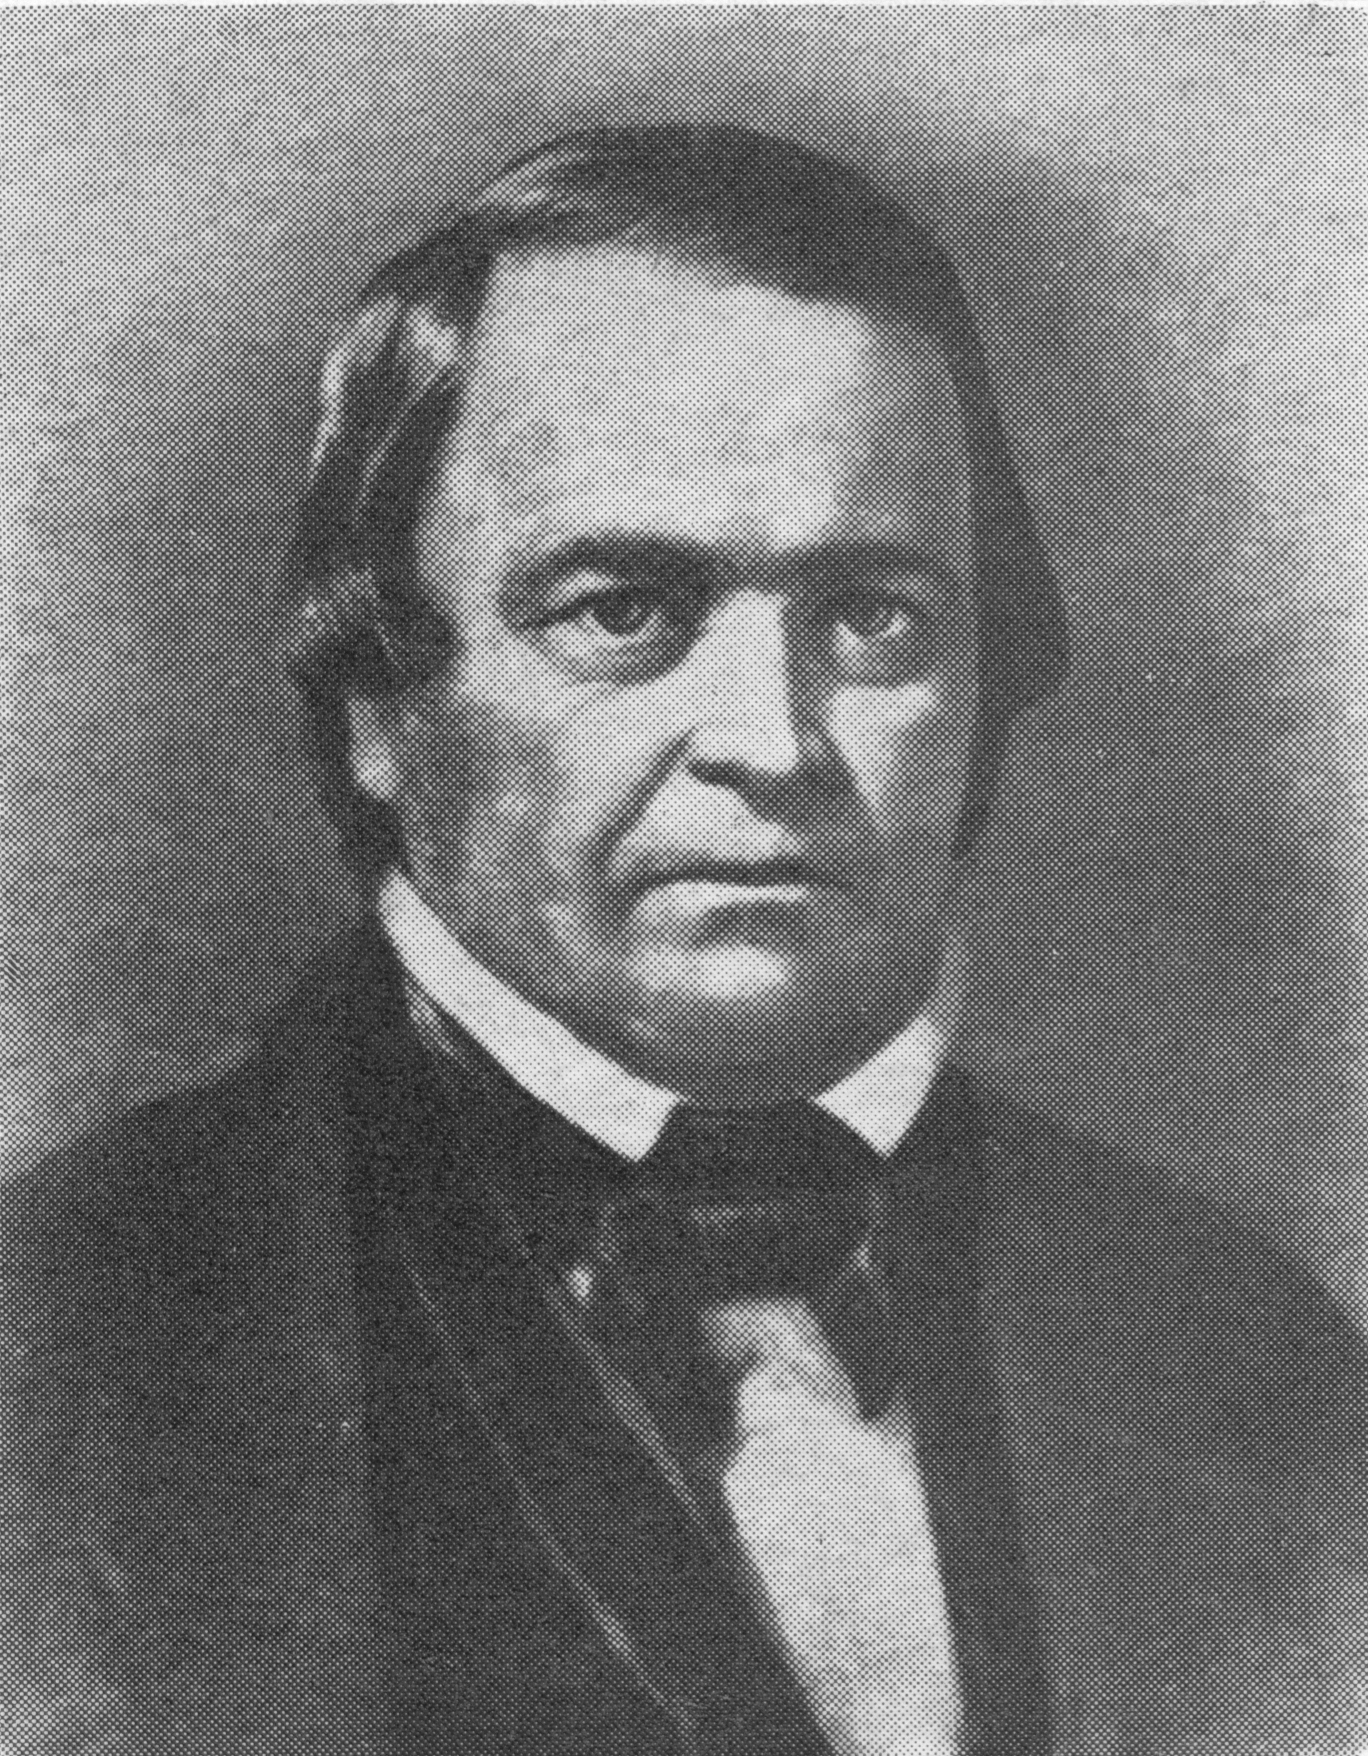
\includegraphics[width=1\linewidth]{images/william-miller.jpg}
    \caption*{William Miller (1782-1849)}
    \label{fig:w-miller}
\end{figure}

Čitajući objašnjenje velikog razočaranja, jeste li primijetili odgovor na pitanje, “\textit{tko je Bog čiji je sud došao}?” Poruka prvog anđela iz Otkrivenja 14:7 točno se podudara s proročkim vremenom objavljenim u Danielu 8:14. Sud koji je došao bio je istražni sud, koji je započeo 1844. Biblija jasno opisuje čiji je čas suda došao u poruci prvog anđela. Pročitajmo to u Bibliji i vidimo komentar Ellen White.

\egw{‘Gledao sam,’ kaže prorok Daniel, \textbf{‘sve dok prijestolja ne bijahu postavljena i \underline{Drevnik vjekova} \underline{ne sjede}}: \textbf{odjeća} mu bijaše bijela kao snijeg, a \textbf{kosa na glavi njegovoj} kao čista vuna; \textbf{prijestolje mu bijaše kao plamenovi ognjeni}, a kotači mu kao rasplamsali oganj. Ognjena je rijeka tekla i izlazila ispred njega; tisuću tisuća služilo je njemu i mirijada mirijadā stajala je pred njim: \textbf{\underline{sud zasjede i knjige se otvoriše}}.’ Daniel 7:9, 10.}[GC 479.1; 1888][https://egwwritings.org/read?panels=p132.2169]

\egwnogap{\textbf{Tako je proroku u viđenju pokazan veliki i svečani dan, u koji će karakter i život svakog čovjeka biti pregledan pred Sucem cijelog svijeta, i kada će svakome biti dano po njegovim djelima. \underline{Drevnik vjekova je Bog Otac}.} Psalmista veli: \textbf{‘Prije} nego što se gore rodiše i prije nego što si sazdao zemlju i svijet, \textbf{od vijeka do vijeka}, \textbf{ti si Bog}.’ Psalam 90:2. \textbf{\underline{On koji je začetnik svega života i izvor svih zakona predsjedavat će na ovome sudu}}. A sveti anđeli kao sluge i svjedoci, na broju ‘tisuće tisuća, i deset tisuća po deset tisuća’, prisustvovat će ovom velikom sudu.}[GC 479.2; 1888][https://egwwritings.org/read?panels=p132.2170]

\egwnogap{\textbf{‘I gle, netko nalik \underline{Sinu Čovječjemu} dolažaše s oblacima nebeskim i dospije do \underline{Drevnika vjekova}, i \underline{dovedoše ga preda nj}}. I njemu bȋ predana vlast i slava i kraljevstvo, da mu služe svi puci, narodi i jezici. Njegova vlast vlast je vječna koja proći neće, i njegovo je kraljevstvo ono koje neće propasti.’ Daniel 7:13, 14. \textbf{Ovdje opisani Kristov dolazak nije njegov drugi dolazak na zemlju}. \textbf{\underline{On dolazi pred Drevnika vjekova na nebu} da primi vlast, slavu i kraljevstvo}, \textbf{koje će mu biti dano na kraju njegove posredničke službe}. \textbf{\underline{Ovaj dolazak, a ne njegov drugi dolazak na zemlju, dogodio se prema proročanstvu na kraju 2300 godina, to jest 1844}}. \textbf{U pratnji nebeskih anđela, naš veliki Svećenik ulazi u svetinju nad svetinjama i dolazi u \underline{Božju prisutnost}} da izvrši posljednje djelo svoje službe za ljude - \textbf{da obavi djelo istražnog suda} i \textbf{izvrši pomirenje} za sve one koji su nađeni dostojni njegove milosti.}[GC 479.3; 1888][https://egwwritings.org/read?panels=p132.2171]

Odgovor je jednostavan i direktan. Bog naših pionira bio je Drevnik Vjekova. \egwinline{Drevnik vjekova je Bog Otac}. On je \textit{osobno}, \textit{duhovno biće}. Vidimo to u njegovom opisu: \bible{Odjeća mu bijaše bijela kao snijeg, a kosa na glavi njegovoj kao čista vuna. Prijestolje mu kao plamenovi ognjeni, a kotači mu kao rasplamsali oganj.}[Daniel 7:9]. Na završetku proročanstva o 2300 dana, u 1844., \bible{dođe čas suda njegova}[Otkrivenje 14:7], dok \bible{Drevnik vjekova ne sjede} i \bible{sud zasjede i knjige se otvoriše.}[Daniel 7:9,10]. Bog iz prve anđeoske poruke je Drevnik vjekova. Naši pioniri nisu bili neupućeni u istinu o Bogu. Vjerovali su \others{Da postoji \textbf{jedan Bog}, \textbf{\underline{osobno, duhovno biće}}, \textbf{stvoritelj svih stvari}, svemoguć, sveznajuć, i vječan, beskonačan u mudrosti, svetosti, pravednosti, dobroti, istini i milosti; nepromjenjiv, i \textbf{\underline{svugdje prisutan po svojem predstavniku, Svetome Duhu}}. Ps. 139:7.}[First point of the Fundamental Principles.] Taj jedan Bog je Otac, Drevnik vjekova, \others{stvoritelj svih stvari}, i mi trebamo \bible{obožavati Onoga koji stvori nebo i zemlju i more i izvore vodne!}[Otkrivenje 14:7]. On \bible{sve stvori po Isusu Kristu}[Efežanima 3:9].

Danas, prva anđeoska vijest nije izgubila ništa od svoje važnosti. Vijesti drugog i trećeg anđela ovise o prvoj vijesti i samo prva vijest zahtijeva akciju s naše strane. Od nas se traži da obožavamo Boga. Točnije, trebamo obožavati pravog Boga. U posljednjem i konačnom sukobu, bit će dvije vrste obožavatelja, kako nam je rečeno u Otkrivenju 13 i 14.

\bible{I poklonit će joj se \textbf{[zvijeri]} svi koji žive na zemlji, \textbf{kojih imena nisu zapisana u Knjizi života Jaganjca} zaklana od postanka svijeta.}[Otkrivenje 13:8]

Grupa koja obožava zvijer primit će žig zvijeri. Cijeli svijet bit će prisiljen obožavati zvijer i njezinu sliku pod prijetnjom smrti.

\bible{I bi joj [zvijeri] dano dati dah \textbf{liku Zvijeri}, tako da i progovori lik Zvijeri i učini da \textbf{tko god se ne pokloni liku Zvijeri bude ubijen}.}[Otkrivenje 13:15]

Ne bismo trebali sudjelovati u tom obožavanju. Potrebno nam je naučiti imati vjeru poput trojice Danijelovih prijatelja koji su odbili obožavati kip kralja Nabukodonozora. Zvijer predstavljena u Otkrivenju 13, koja ucjenjuje savjesti ljudi pod prijetnjom njihovih života, je papinstvo. Dragi prijatelju, ne daj se prevariti. Bog papinstva je Bog Trojstva. Nemoj to zanemariti.

Trebali bismo obožavati Drevnika Vjekova kako je to objavljeno u prvoj anđeoskoj poruci. To je Bog Stvoritelj koji je sve stvorio preko Svog Sina, Isusa Krista. To je Bog iz prve točke \emcap{Fundamentalnih Principa}. Naši pioniri su imali ispravno razumijevanje.

Istinsko razumijevanje misije i svrhe pokreta Adventista Sedmoga Dana trebalo bi biti konačan dokaz da je doktrina Trojstva strana doktrina za nas. Završili smo tu gdje smo danas jer smo zaboravili \egwinline{\textbf{kako nas je Gospodin vodio i \underline{Njegovo učenje} u našoj prošlosti.}}[LS 196.2; 1915][https://egwwritings.org/read?panels=p41.1083] Vrlo je tužno vidjeti kako naši adventistički povjesničari i teolozi tvrde da naši pioniri nisu ispravno razumjeli doktrinu o Bogu. Da je to istina, naši pioniri ne bi uspjeli proglasiti prvu anđeosku vijest. Oni nisu promašili svrhu svojeg postojanja, no nažalost, izgleda da mi jesmo.

\others{\textbf{Većina osnivača Adventizma Sedmog dana danas ne bi mogla pristupiti crkvi ako bi morali pristati na denominacijska Osnovna Vjerovanja}.}\others{\textbf{Konkretnije, većina se ne bi mogla složiti s vjerovanjem broj 2, koje se bavi doktrinom o Trojstvu.} Za Josepha Batesa Trojstvo je bila nebiblijska doktrina, za Jamesa Whitea to je bila ‘ona stara trinitarijanska apsurdnost’, a za M. E. Cornella to je bio plod velike otpadnosti, zajedno s takvim lažnim doktrinama kao što su čuvanje nedjelje i besmrtnost duše.}[George Night, Ministry Magazine, October 1993][https://www.ministrymagazine.org/archive/1993/10/adventists-and-change]

Doktrina o Trojstvu je doktrina koja potkopava temelj naše vjere, temelj koji je postavljen na početku našeg djelovanja. Razlika između istine i zablude leži u hermeneutici—metodi tumačenja Biblije. U sljedećem poglavlju, temeljito ćemo istražiti ovu problematiku.

% Prisjećanje početka

\begin{titledpoem}

    \stanza{
        Sjećanje na početak, vjere naše trag, \\
        Pioniri su slijedili istine prag. \\
        Godine 1844. došao je sud, \\
        Drevnik vjekova sjeo je, to bijaše čud.
    }

    \stanza{    
        Danas se pitamo tko je Bog pravi, \\
        Kojeg prvi anđeo jasno objavi. \\
        Ako su pioniri bili u krivu tada, \\
        Cijela njihova misija u vodu pada.
    }

    \stanza{    
        Danas se mijenja što nekad je bilo, \\
        Trojstvo se uvuklo, istinu skrilo. \\
        Vratimo se vjeri koja nas je stvorila, \\
        Da bi nas istina Božja oslobodila.
    }
    
\end{titledpoem}